
%(BEGIN_QUESTION)
% Copyright 2008, Tony R. Kuphaldt, released under the Creative Commons Attribution License (v 1.0)
% This means you may do almost anything with this work of mine, so long as you give me proper credit

Derivatvirkning kan ikke brukes i prosesser der PV-signalet inneholder mye {\it støy}, slik som vist i denne trenden:

$$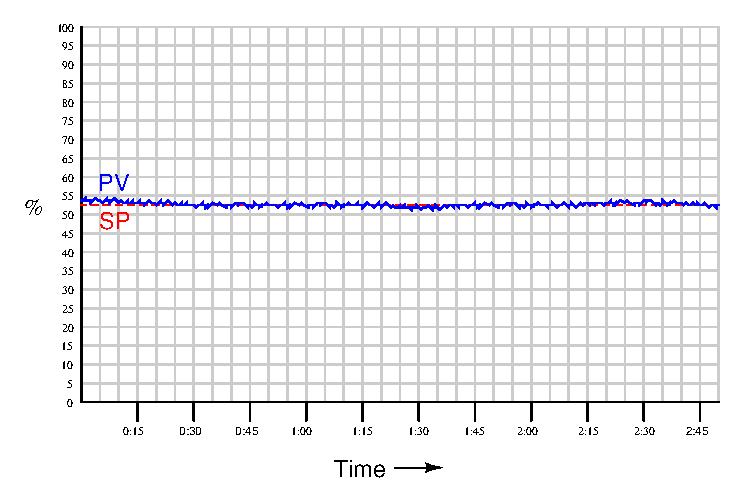
\includegraphics[width=15.5cm]{i01671x01.eps}$$

Forklar hvorfor støy og derivatkontroll er uforenlige.

Avgjør også om {\it integralvirkning} påvirkes av støy i PV-signalet på samme måte, og forklar svaret ditt.

\underbar{file i01671}
%(END_QUESTION)





%(BEGIN_ANSWER)

Derivatdelen ser på *endringshastigheten*. Støy består av mange små, men veldig raske endringer (høy frekvens). Derfor vil derivatdelen forsterke støyen enormt og gi en svært urolig regulatorutgang, noe som sliter på ventiler og utstyr.

Integralvirkningen derimot, ser på *arealet* under kurven (akkumulert feil). Siden støy svinger raskt frem og tilbake rundt den sanne verdien, vil de positive og negative bidragene kansellere hverandre ut over tid. Derfor påvirkes integralvirkningen svært lite av støy.

%(END_ANSWER)





%(BEGIN_NOTES)

Dette er grunnen til at D-delen sjelden brukes i strømningsregulering (flow control), som ofte er beheftet med turbulensstøy.

%INDEX% Control, derivative: noisy process signal
%INDEX% Control, integral: noisy process signal

%(END_NOTES)
